%
%
%


\chapter{Rotational Dynamical Systems}

\section{Problem Statement and Learning Objectives}

\begin{itemize}
  \item System Elements \& constitutive relations.
  \item Equations of Motion
  \item Gears
  \item Conversion to Transfer Function
\end{itemize}

\section{System Elements \& constitutive relations.}

Rotation is a different type of motion than translation and it makes subtle differences in dynamic analysis.   One of the most prominent difference is that if a body is rotating, every point in the body has a different velocity and acceleration.   This complex situation can be considerably simplified by assuming a single axis of rotation, and representing a body by its {\it inertia} instead of its mass.   The axis of rotation is a line along which points in a rigid body do not move when it is rotated about the axis.  

Computation of the inertia of a rigid body is beyond the scope of this book, but it is a quantity which can be measured by rotational tests, or calculated from information such as a CAD model.  

\subsection{Torque}

{\it Torque} (also called {\it moment}) is a vector quantity relating a force and an associated {\it moment arm} through which the force acts to rotate a body around an axis.   The simplest case is a force which is perpendicular to both the axis of rotation and a radius connecting the axis and the point through which the force is acting on the rigid body (Figure \ref{forceradisutorque}, Left). In this case, the magnitude of the torque is 
\[
|\tau| = |r||F|
\]
and the full magnitude and direction of the torque vector will be obtained by the right hand rule
\[
\tau = r \times F
\]
(where $\times$ indicates the vector cross product.

If the force vector is not applied at a right angle (Figure \ref{forceradisutorque}, Right), it must be resolved into  perpendicular and radial components, $F_p, F_r$, and then the torque magnitude is
\[
|\tau| = |r||F_p|
\]
the full torque vector can still be obtained by the vector cross product above.   When the axis of rotation is fixed, for example by a shaft mounted in bearings, then only the component of the torque vector which is parallel to the axis causes rotation about the axis. 

In most of the problems we will study however, we will assume that a torque value is a known or measured quantity and not worry about the radius or moment arm.  In a very common control system application, a DC electric motor is applied to a shaft and the torque is simply proportional to the current 
\[
\tau(t) = K_m i(t)
\]

\begin{figure}\centering
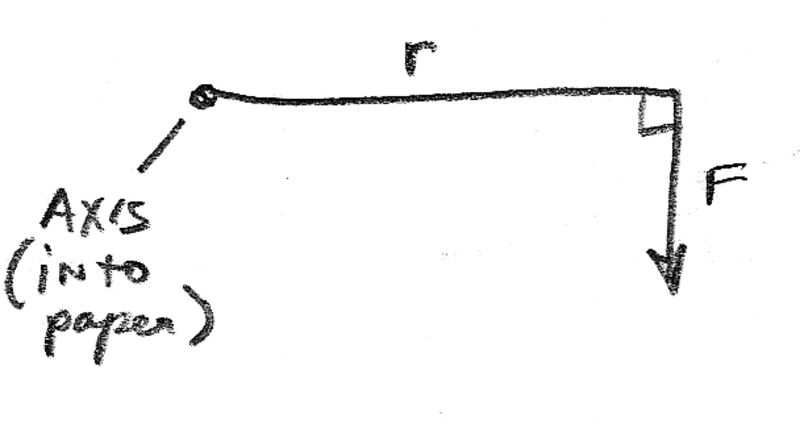
\includegraphics[width=2.0in]{figs03/00749.png} \hspace{0.75in}
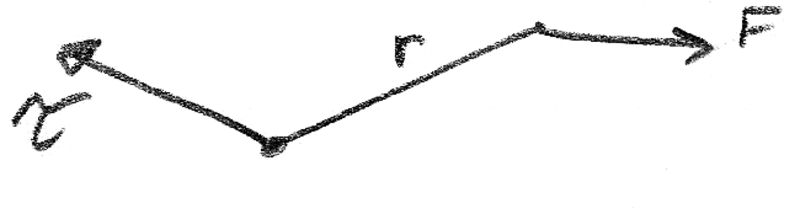
\includegraphics[width=2.0in]{figs03/00750.png}
\caption{An applied force $F$ generates a torque if it acts through a point having a radius, $r$ from the axis of rotation. Left: force is applied perpendicular to the moment arm. Right: force is appled in a general direction. (see text).}\label{forceradisutorque}
\end{figure}


















\subsection{Elements of Rotational Dynamical Systems}
We will analyze systems consisting of 
\begin{itemize}
  \item {\bf Inertia}     The property of a rigid body which resists angular acceleration, and which stores kinetic energy. 
  \item {\bf Stiffness}   The property of a rigid body which resists angular displacement, and which stores potential energy. 
  \item {\bf Damping}     The property of a rigid body which resists change in angular displacement and which converts motion to heat. 
\end{itemize}


Some properties of the various elements are summarized Table \ref{RotElementsTable}.


\begin{table}
\begin{tabular}{|l|l|l|l|p{2.5in}|} \hline
 Name             &  Physical Realization        &   Symbol    &  Equation              & Notes   \\ \hline
  Inertia         &  Flywheel                    &   $J$ 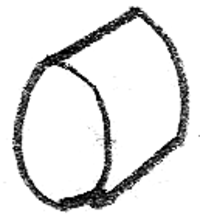
\includegraphics[width=0.5in]{figs03/00740a.png}     &  $\tau(t) = J\ddot{\theta}$    &  \\ \hline
  Stiffness       &  Coil  Spring                &       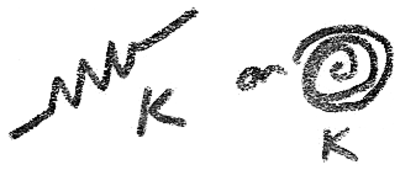
\includegraphics[width=1.0in]{figs03/00740b.png}    &  $\tau(t) = K{\theta}$         & $\tau$ is same on both sides.  Assume zero rest length \\ \hline 
  Damping         & Fan, rotary damper, friction &       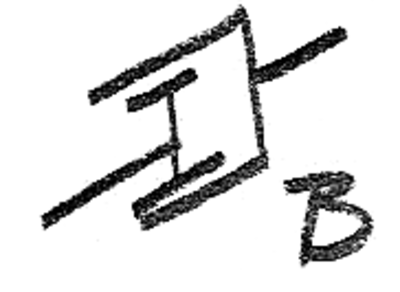
\includegraphics[width=1.0in]{figs03/00740c.png}    &  $\tau(t) = B\dot{\theta}$     & This is a linear model for friction.     \\ \hline
\end{tabular}\caption{}\label{RotElementsTable}
\end{table}



\section{Equations of Motion}
Similarly to translational motion (see Equation \ref{D'Alembert}), there is an Equation of Motion (EOM) for each inertia in the system:
\[
J\ddot{theta} + \sum_j B_j(\dot{\theta} -\dot{\theta}_j) + \sum_kK(\theta-\theta_k)
\]

The use of this EOM is similar to that of translational dynamical systems as illustrated in the following examples

\begin{ExampleSmall}
Find the equation or equations of motion for the following system 

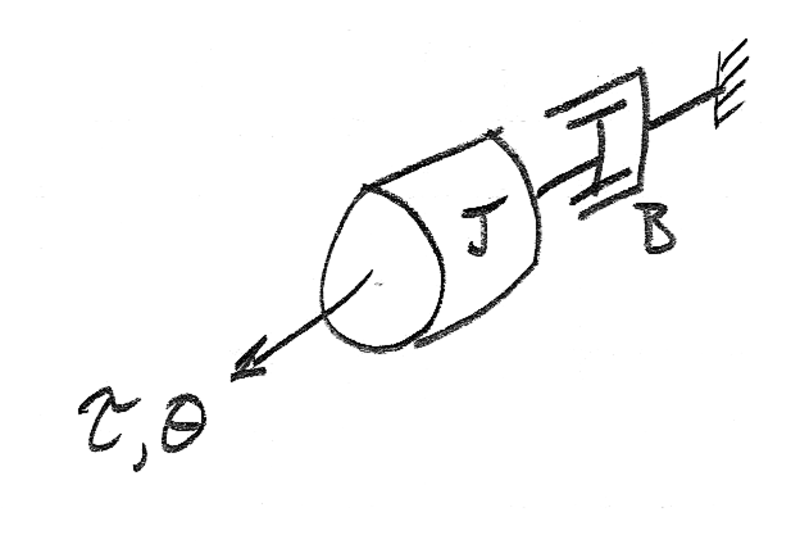
\includegraphics[width=2.0in]{figs03/00741.png}

There is one inertia ($J$) so there is only one EOM:
\[
J\ddot{\theta} + B(\dot{\theta}-0) = \tau(t)
\]
or
\[
J\ddot{\theta} + B\dot{\theta} = \tau(t)
\]
\end{ExampleSmall}


\begin{ExampleSmall}
Find the equation or equations of motion for the following system 

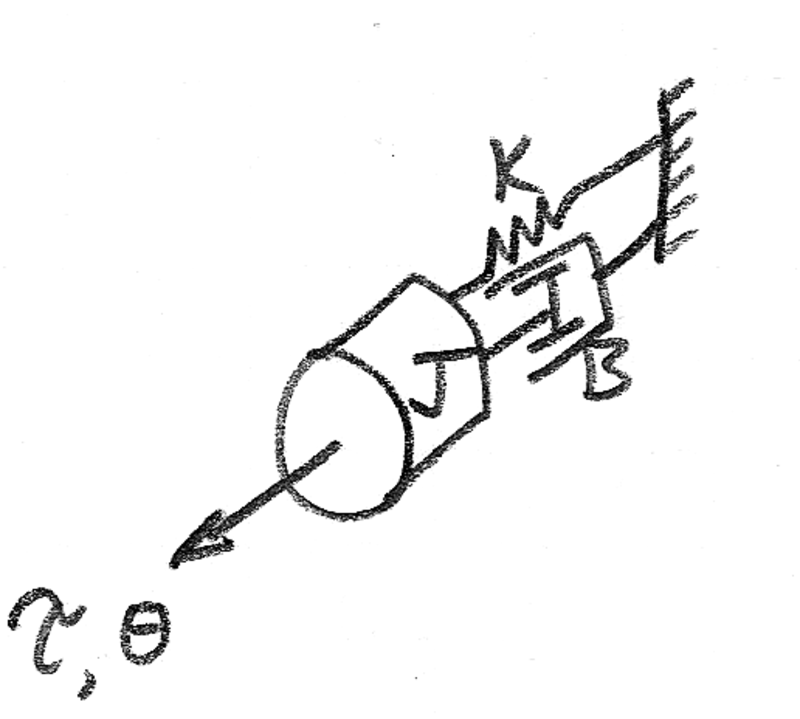
\includegraphics[width=2.0in]{figs03/00742.png}

There is still only one EOM but it has an additional spring element:

\[
J\ddot{\theta} + B(\dot{\theta}-0) + K(\theta-0 = \tau(t)
\]
or
\[
J\ddot{\theta} + B\dot{\theta} + K\theta = \tau(t)
\]

\end{ExampleSmall}


\begin{ExampleSmall}
Find the equation or equations of motion for the following system 

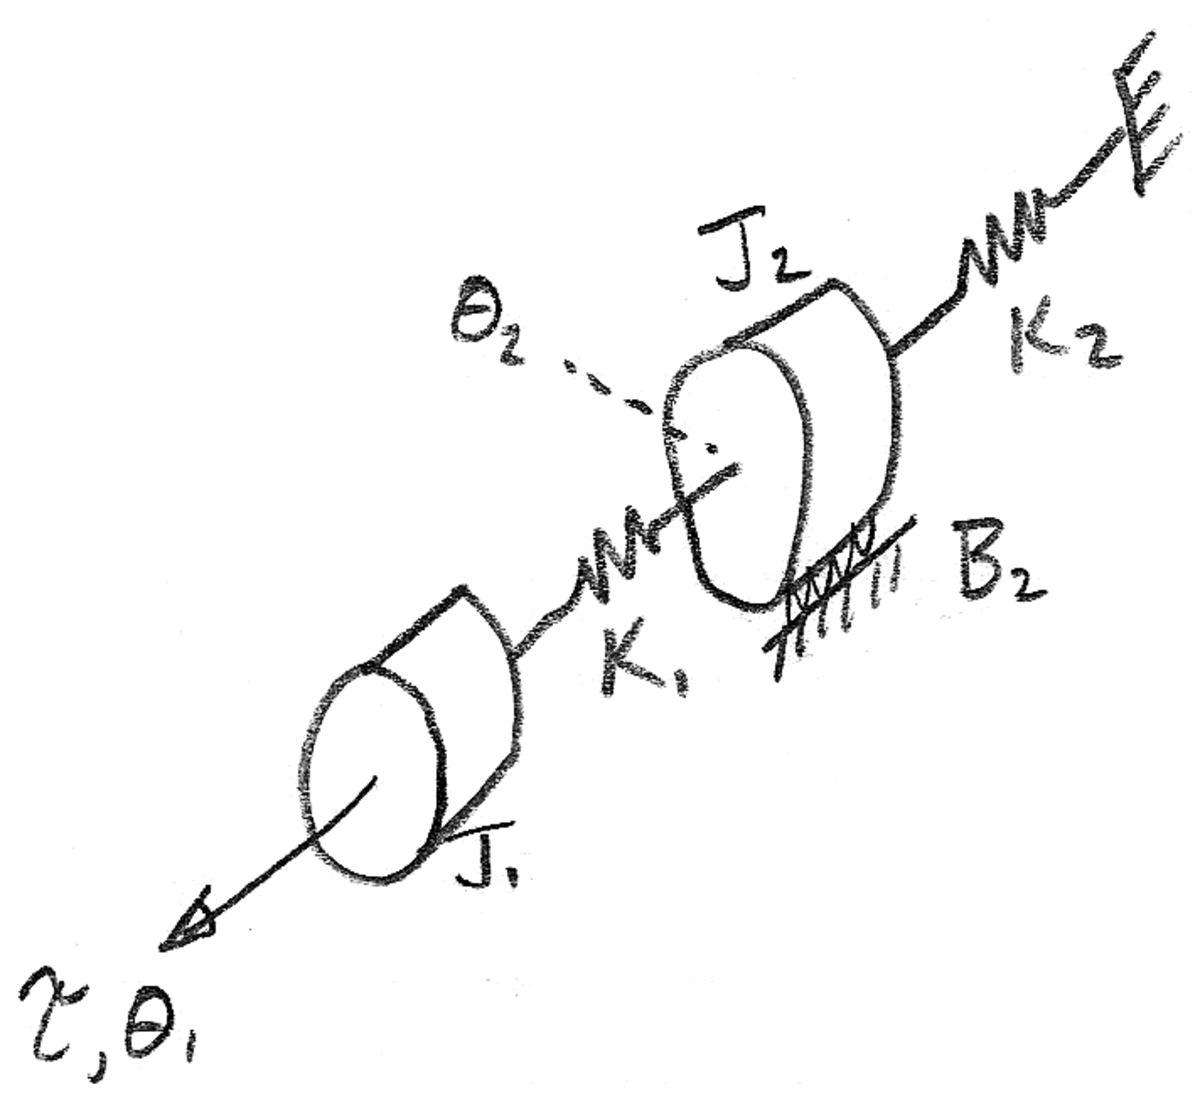
\includegraphics[width=3.0in]{figs03/00743.png}

This system has two masses.  Although they appear to be on the same axis, they are separated by a spring and thus they can have different displacements depending on the deflection of the spring.  As a result we have two EOM:

\[
J_1\ddot{\theta} + K_1(\theta_1 - \theta_2) = \tau(t)
\]
\[
J_2\ddot{\theta} + K_1(\theta_2 - \theta_1) + K_2\theta_2 + B_2\dot{\theta_2} = 0
\]
These usually need to be solved simultaneously as with translational systems. 

\end{ExampleSmall}

Once the OEMs are available, transfer functions can be derived in the same way as with translational systems.

\section{Gears}

\begin{figure}[h]\centering
\includegraphics[width=2.5in]{figs03/gear-spur_Emerson.jpg}
\caption{Meshing spur gears ({\tt http://www.emersonindustrial.com/}).}\label{2meshedgears}
\end{figure}

\subsection{Gear Kinematic Relationships}\label{gearkinematics}

A common system element in rotary systems is gears.  The corresponding element in translational systems, levers, seem to appear less often in control systems. 

Consider two meshed gears, gear 1 and gear 2 (Figure \ref{2meshedgears}).  
Each gear has $N_i$ teeth.    
The size of each tooth is $2\pi r_i/ N_i$.  The number of teeth which pass when a gear is rotated by $\theta_i$ is $N_i\frac{\theta_i}{2\pi}$.
Since the teeth must be the same size for the gears to mesh, we can write
\[
\frac{N_1\theta_1}{2\pi} = \frac{N_2\theta_2}{2\pi}
\]
or
\[
\frac {\theta_1}{\theta_2}  =  \frac{N_2}{N_1}
\]
differentiating we also have
\[
\frac { \dot{\theta}_1}{ \dot{\theta_2}}  =  \frac{N_2}{N_1} \qquad 
\frac {\ddot{\theta}_1}{\ddot{\theta_2}}  =  \frac{N_2}{N_1}
\]

\begin{figure}\centering
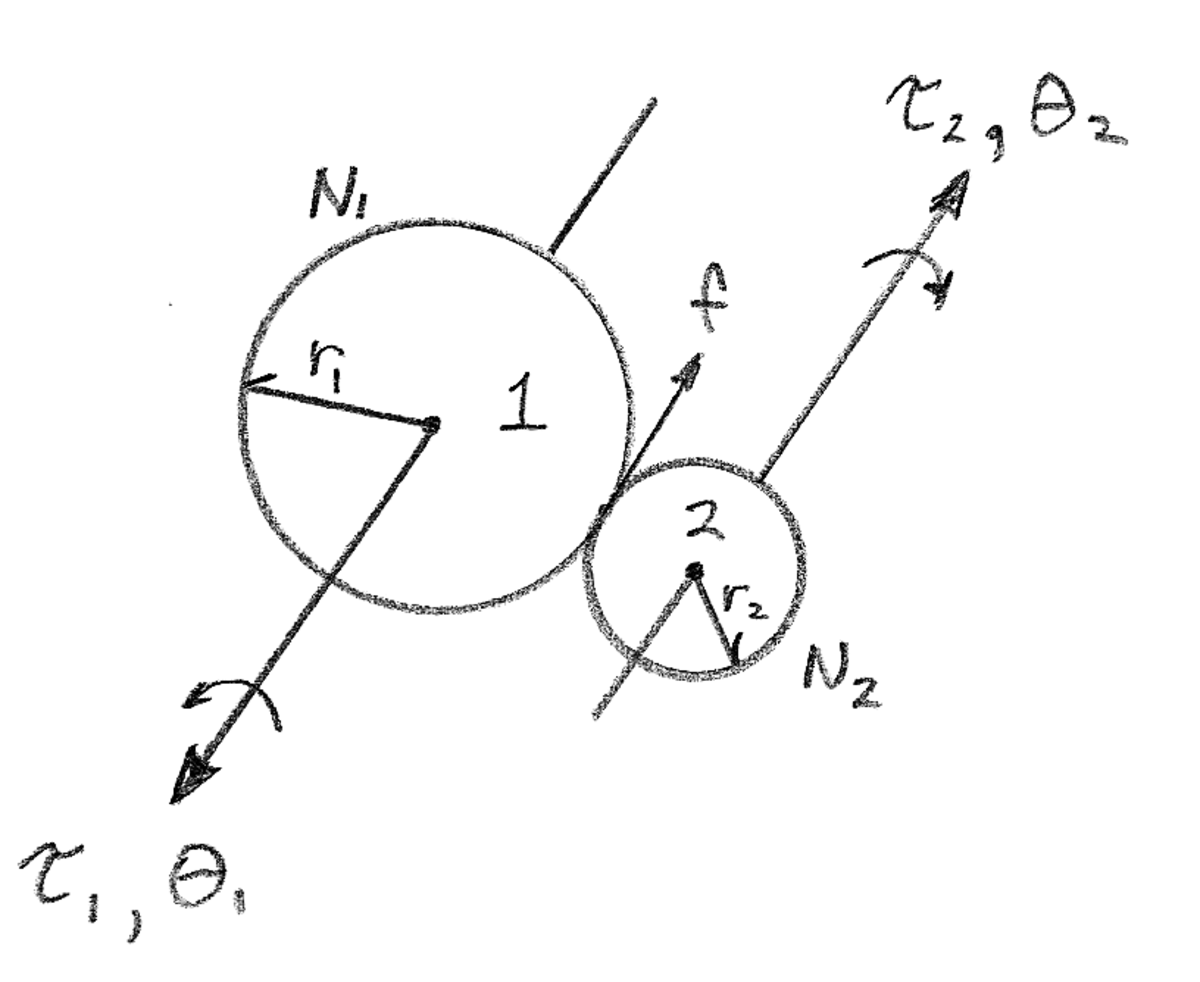
\includegraphics[width=3.0in]{figs03/00744.png}
\caption{Two meshed gears.}\label{2meshedgears}
\end{figure}

Commonly we define $n  = N_1/N_2$.   Thus
\[
\dot{\theta_2} = n \dot{\theta_1}
\]
etc. 


There is a force exerted by one tooth on the other in the tangential direction, $f$ (Figure \ref{2meshedgears}).  Since it is tangential, we can relate it easily to the torques:
\[
\tau_1 = r_1f \qquad \tau_2 = r_2f
\]
This gives 
\[
\tau_1 = \frac{r_1}{r_2}\tau_2 = n\tau_2
\]
\[
\tau_2 = \frac{1}{n} \tau_1
\]

\subsubsection{Simplification of Geared Systems}

We can use the properties of gear transmission of rotation and torque to simplify the process of writing EOM.

Consider a damper driven by a set of gears (Figure \ref{dampergears})

\begin{figure}\centering
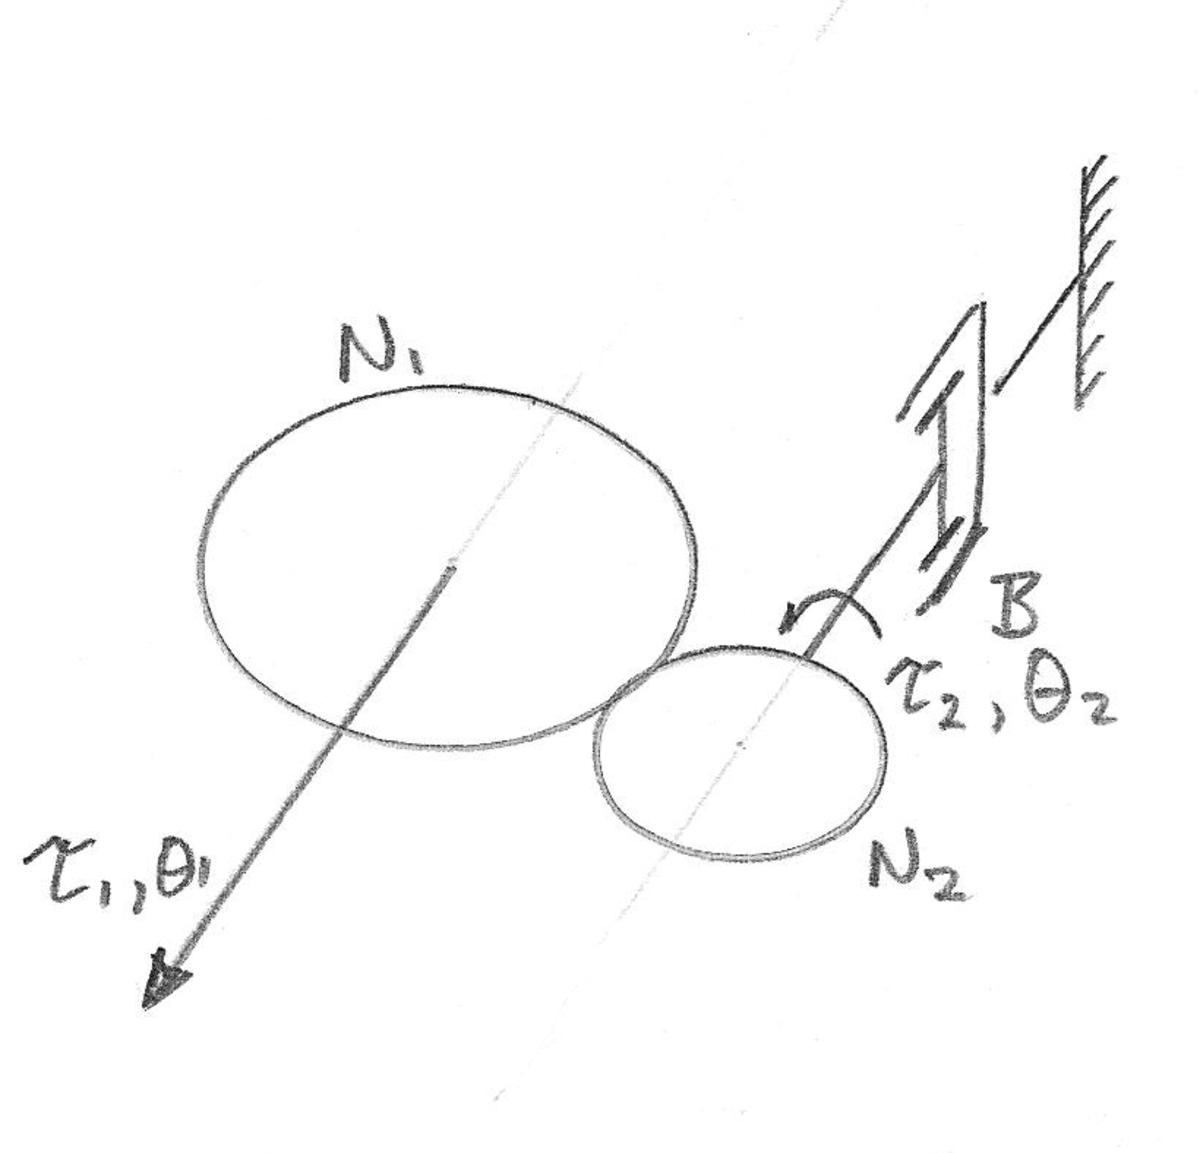
\includegraphics[width=3.0in]{figs03/00745.png}
\caption{A viscous load (damper) driven by a set of gears.}\label{dampergears}
\end{figure}

We have
\[
\tau_2 = B \dot{\theta_2}
\]
Using the relationships above we have
\[
\frac{1}{n}\tau_1 = Bn\dot{\theta}_1
\]
or
\[
\tau_1 = Bn^2\dot{\theta}_1
\]

Suppose the system ``beyond" the gears had some mass and spring in addition to the damper of Figure \ref{dampergears}. The argument above would be very similar: 

We have
\[
\tau_2 = J \ddot{\theta}_2 + B \dot{\theta}_2 + K \theta_2
\]
Using the relationships above we have
\[
\frac{1}{n}\tau_1 =J n \ddot{\theta}_1 + B n\dot{\theta}_1 + K n\theta_1
\]
or
\[
\tau_1 =J n^2 \ddot{\theta}_1 + B n^2\dot{\theta}_1 + K n^2\theta_1
\]

Let 
\[
\hat{J} = n^2J \qquad \hat{B} = n^2B \qquad \hat{K} = n^2 K
\]
The EOM becomes
\[
\tau_1 =\hat{J}\ddot{\theta}_1 + \hat{B} \dot{\theta}_1 + \hat{K} \theta_1
\]
This is the EOM of a simpler system (Figure \ref{simplifiedgearsys}). 

\begin{figure}\centering
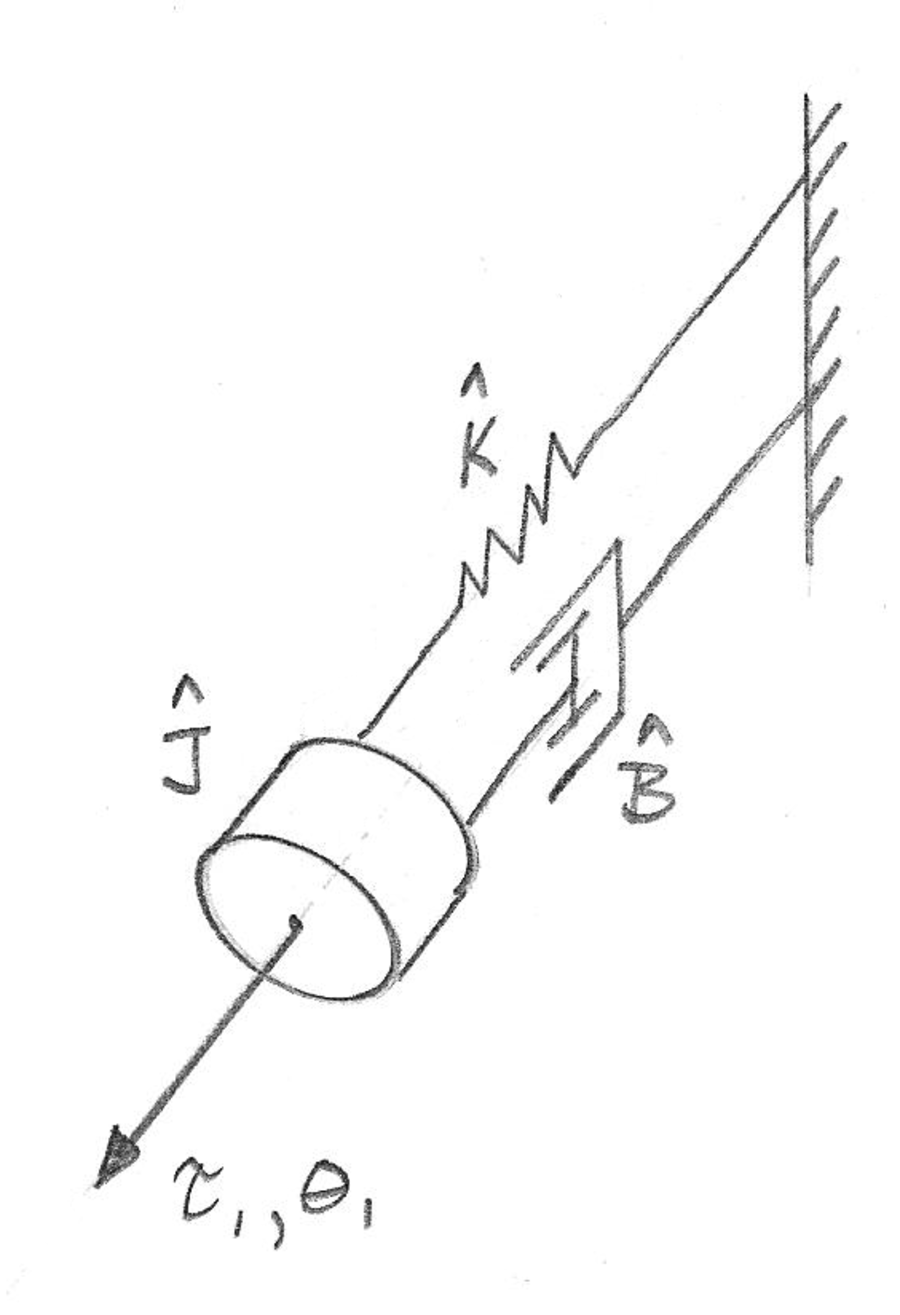
\includegraphics[width=2.25in]{figs03/00746.png}
\caption{Simplified equivalent system of the system in Figure \ref{dampergears}}\label{simplifiedgearsys}
\end{figure}



\begin{ExampleSmall}
Transform the following geared system into an equivalent non-geared system and write the EOM. 

\begin{tabular}{p{2.5in}p{2.5in}}
\vtop{\vskip-2ex \hbox{ 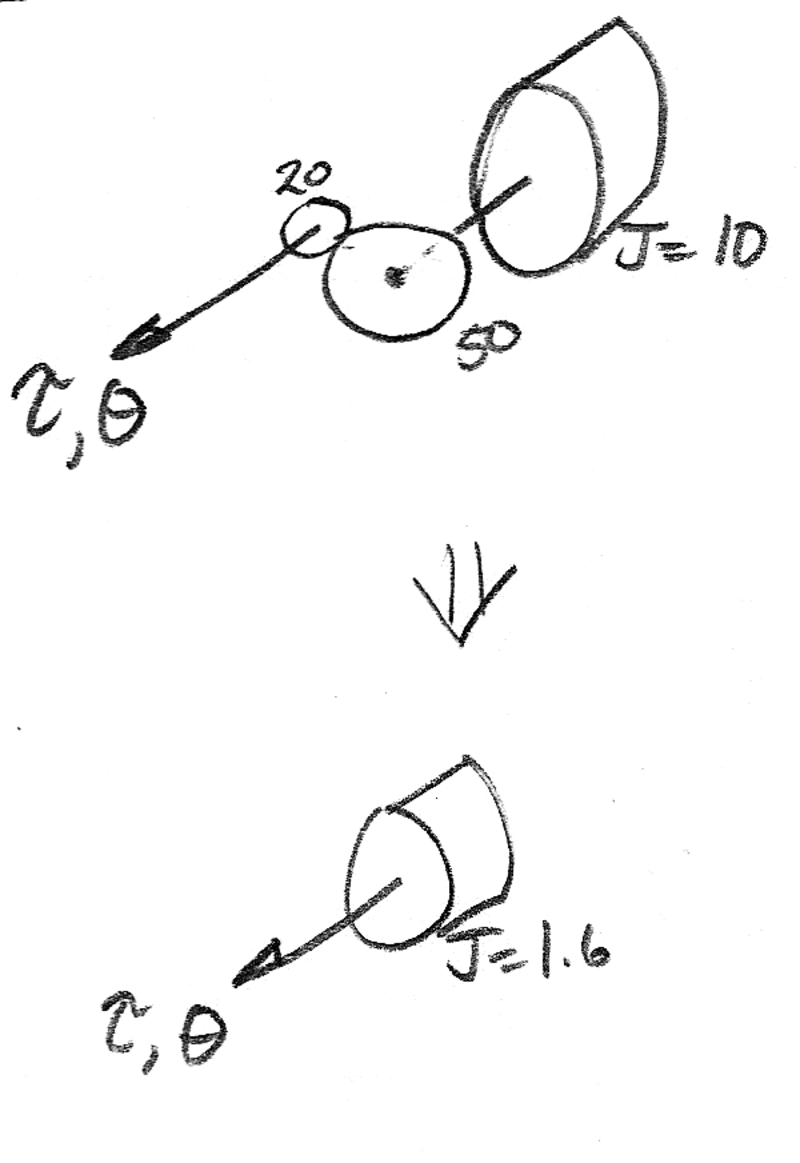
\includegraphics[width=2.0in]{figs03/00747.png}  }}
&
\[
n = \frac {20}{50} = 0.4
\]
\[
\hat{J} = 0.4^2J = 0.16\times 10 = 1.6
\]
\[
\tau = 1.6\ddot{\theta}
\]
\end{tabular}

\end{ExampleSmall}


\begin{ExampleSmall}
Transform the following system into an equivalent system without gears

\begin{tabular}{cp{2.5in}}
\vtop{ \vskip-2ex  \hbox{  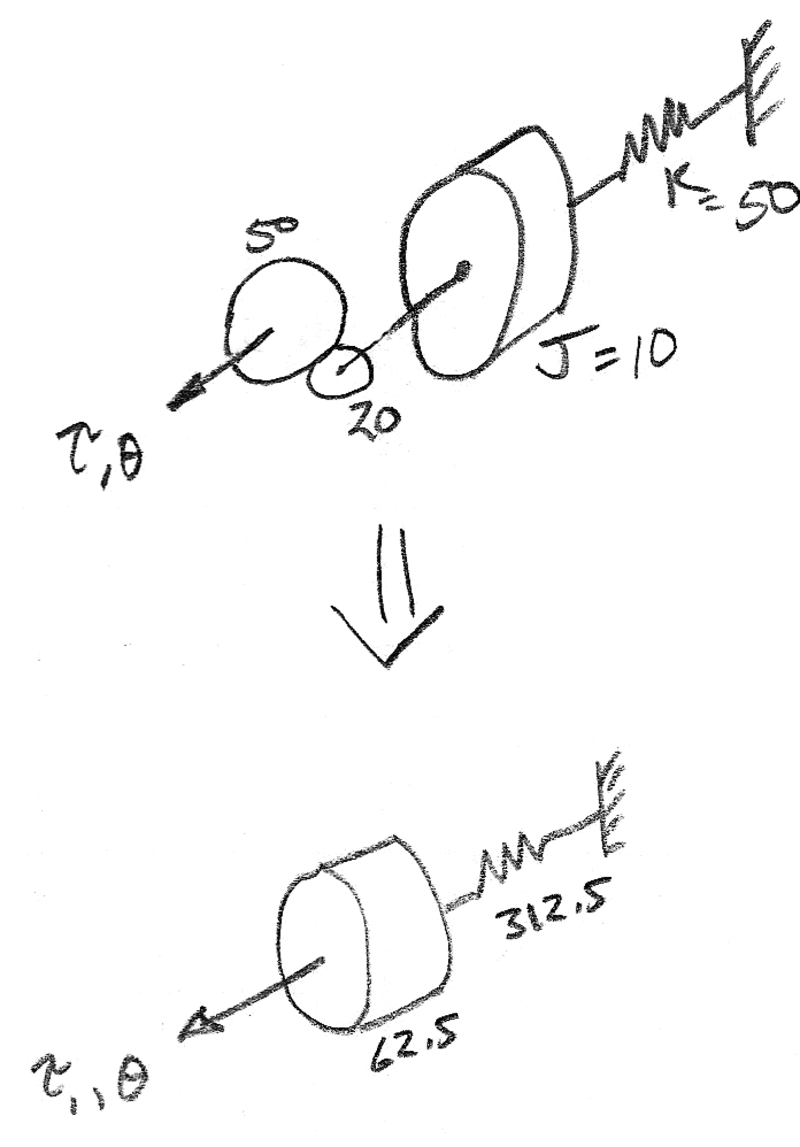
\includegraphics[width=2.0in]{figs03/00748.png}  }}
&
\[
n = \frac {50}{20} = 2.5
\]
\[
\hat{J} = 2.5^2\times 10 = 62.5 
\]
\[
\hat{K} = 2.5^2\times 50 = 312.5 
\]

\[
\tau = 62.5\ddot{\theta} + 312.5\theta
\]
\end{tabular}

\end{ExampleSmall}


\begin{Example}
Transform the following system with two rotational inertias and gears to eliminate the gears, and then write and solve EOMs to get the transfer function
\[
G(s) = \frac {\theta_2(s)} {\tau(s)}
\]

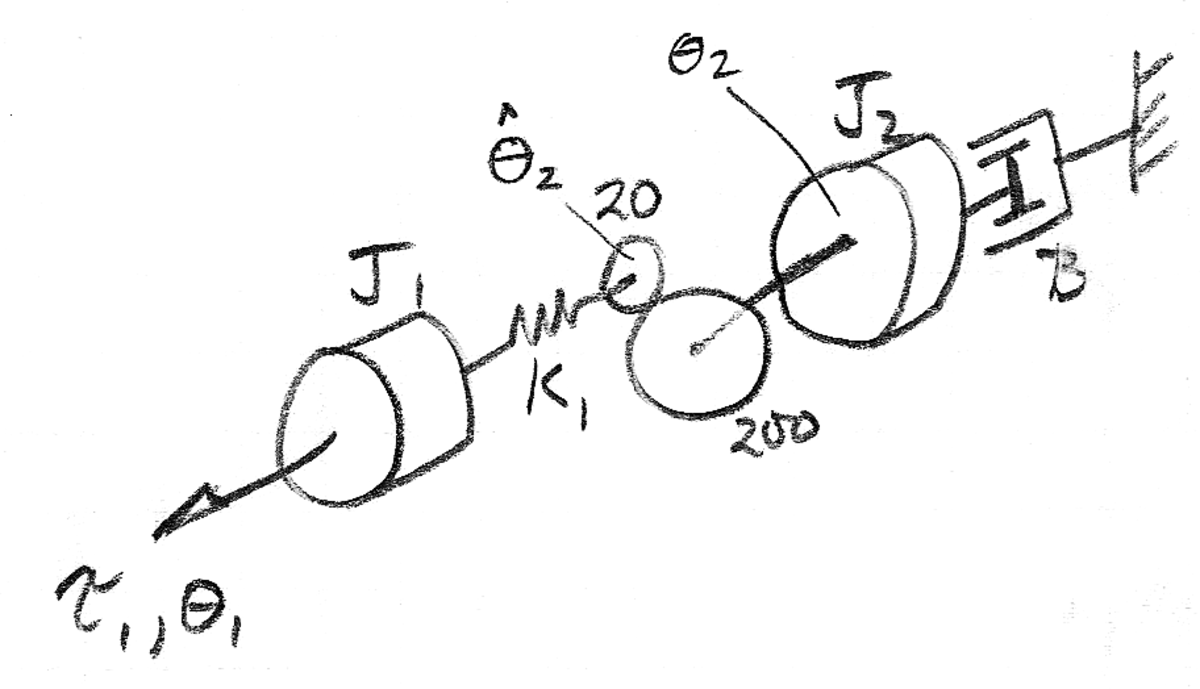
\includegraphics[width=3.0in]{figs03/00751.png}  

First, develop the transformations (by $n^2$) to change $J_2$ and $B_2$ so as to eliminate the gear set:
\[
n = \frac{20}{200} = 0.1, \quad n^2 = 0.01 
\]
\[
\hat{J}_2 = 0.01 J_2 \qquad  \hat{B} = 0.01B
\]
Also, the displacement of the second inertia is changed by
\[
\hat{\theta}_2 = \frac{1}{n}\theta_2 = 10\theta_2
\]
Note that the displacement $\theta_2$ is transformed differently from the elements $J_2,B_2$ according to the derivations in Section \ref{gearkinematics}. 
Also note that $\hat{\theta}_2$ is not the same as $\theta_1$ because the spring $K_1$ can have an arbitrary deformation. 

The transformed system is 

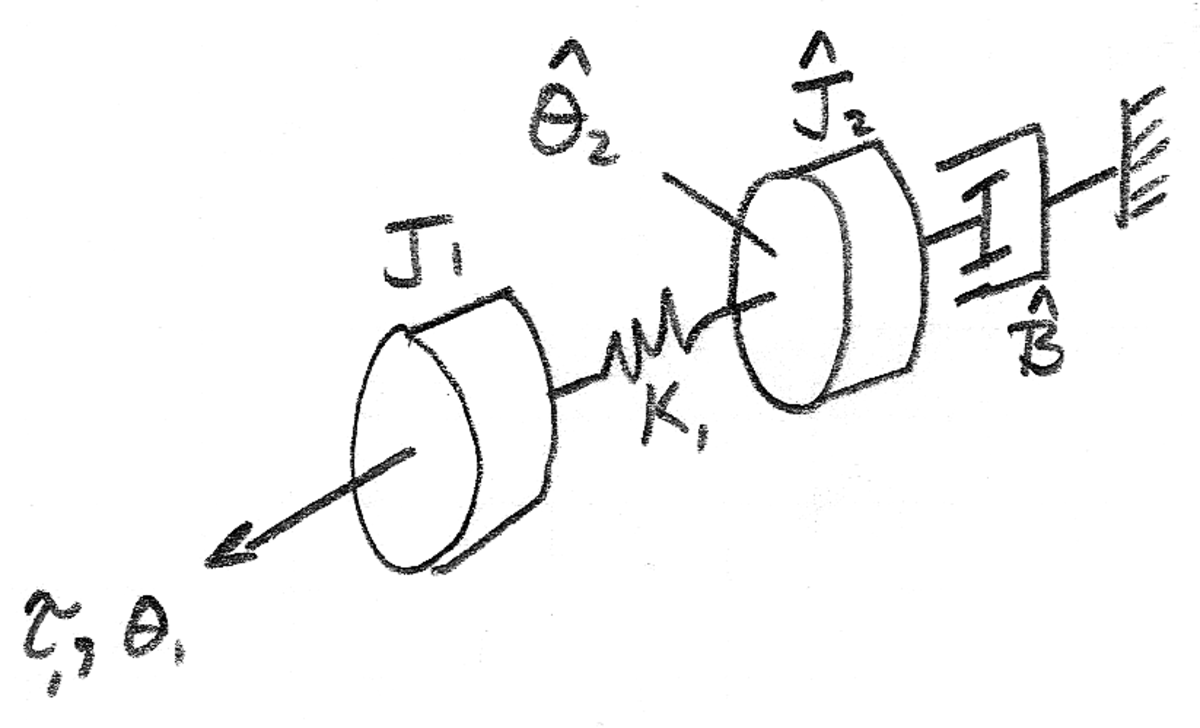
\includegraphics[width=3.0in]{figs03/00752.png}  


\end{Example}

\begin{ExampleCont}

Solving, using the techniques in Chapter 2:

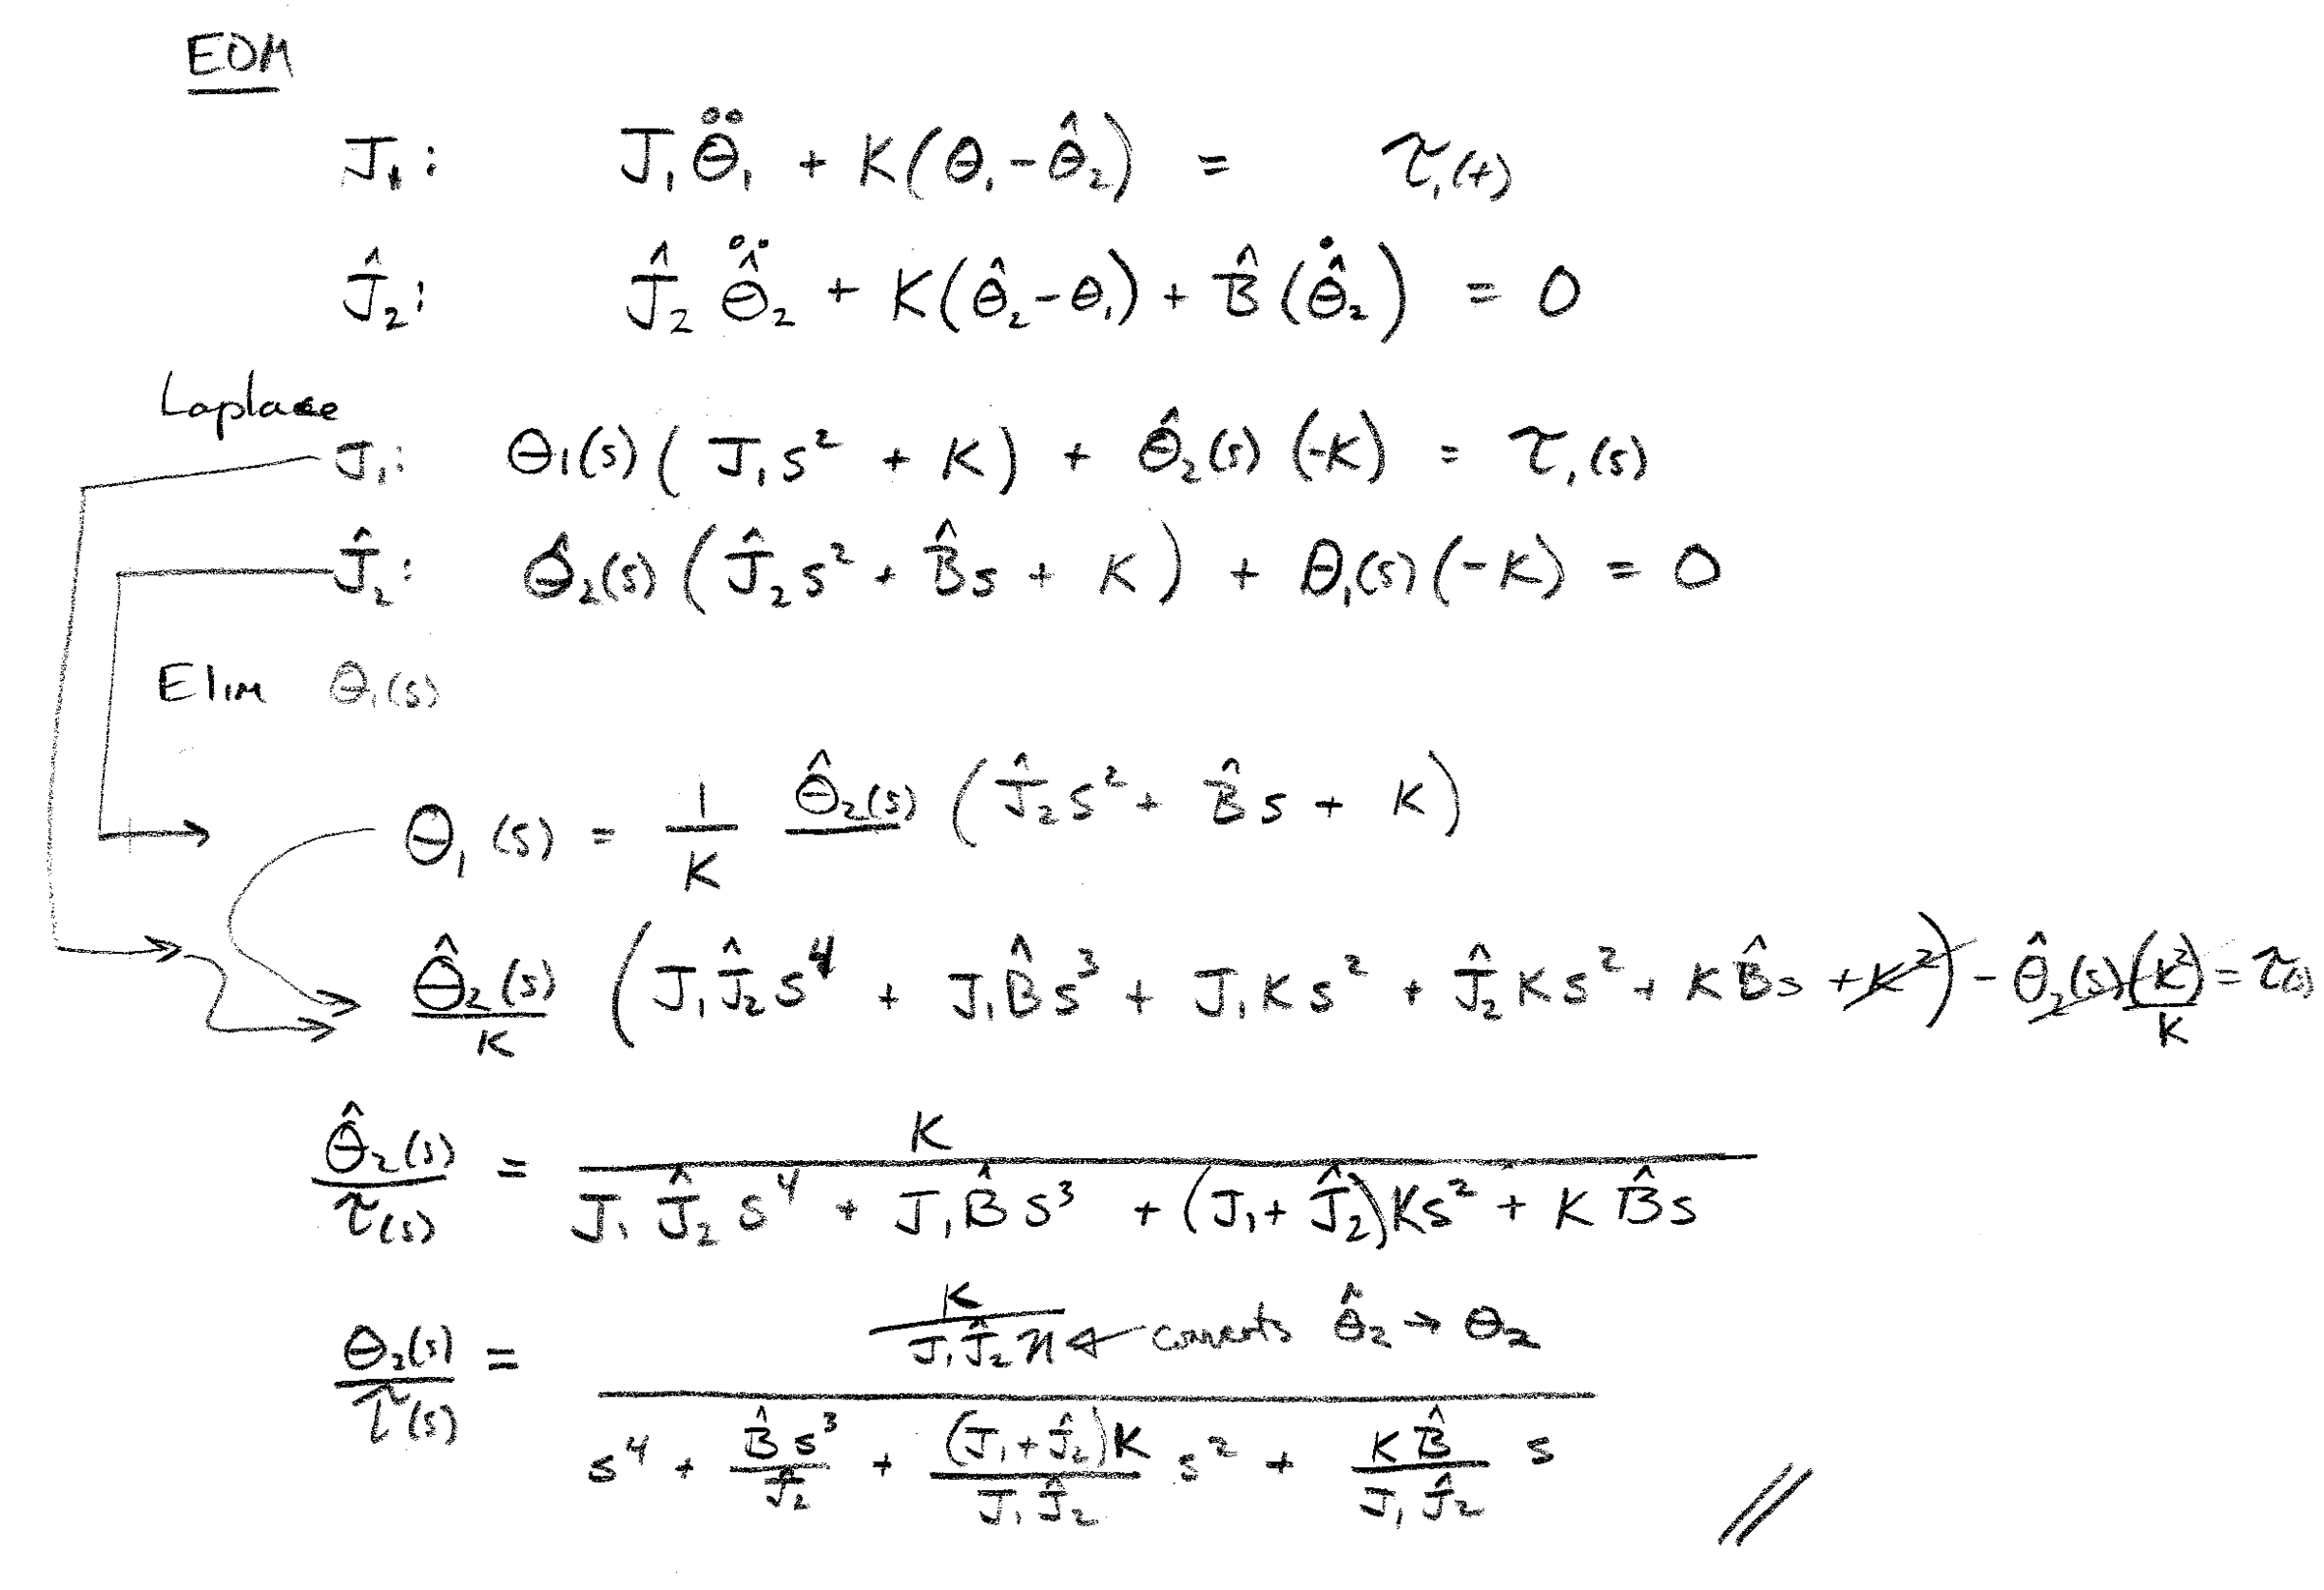
\includegraphics[width=6.0in]{figs03/00753.png}  

\end{ExampleCont}


\section{Rotary to Linear Motion} 

\begin{figure}\centering
\includegraphics[width=2.5in]{figs03/stober_rack_pinion.jpg}
\caption{Rack and Pinion drive system (Stober, {\tt www.stober.com})}\label{stoberrackpinion}
\end{figure}

Sometimes the second gear in a chain is straightened out to $r_2 = \infty$.  The case of infinite radius corresponds to what is called a {\it rack} - a set of gear teeth arrayed in a straight line.  The gear which meshes with a rack is called a {\it pinion} (Figure \ref{stoberrackpinion}).  Such systems contain a combination of rotating and translating elements and they can be analyzed by careful application of the principles developed in this and the previous chapters.  

Consider the rack and pinion shown in Figure \ref{rackpinion}.  Assume the gear can rotate about it's fixed axis and the rack is free to slide back and forth in the $x$ direction.  The force applied by the rack to the gear must be 
\[
F = \tau/r
\]
because of the tangential contact constraint.   The displacements are related by
\[
x = r\theta
\]
by the basic geometry of circles. 

In a combined system we write translational EOM(s) for the sliding components and rotational EOM(s) for the rotating components, but by substituting the relationships above, we can transform one of the EOMs so that both are in terms of rotary (or translational) variables. 

 


\begin{figure}\centering
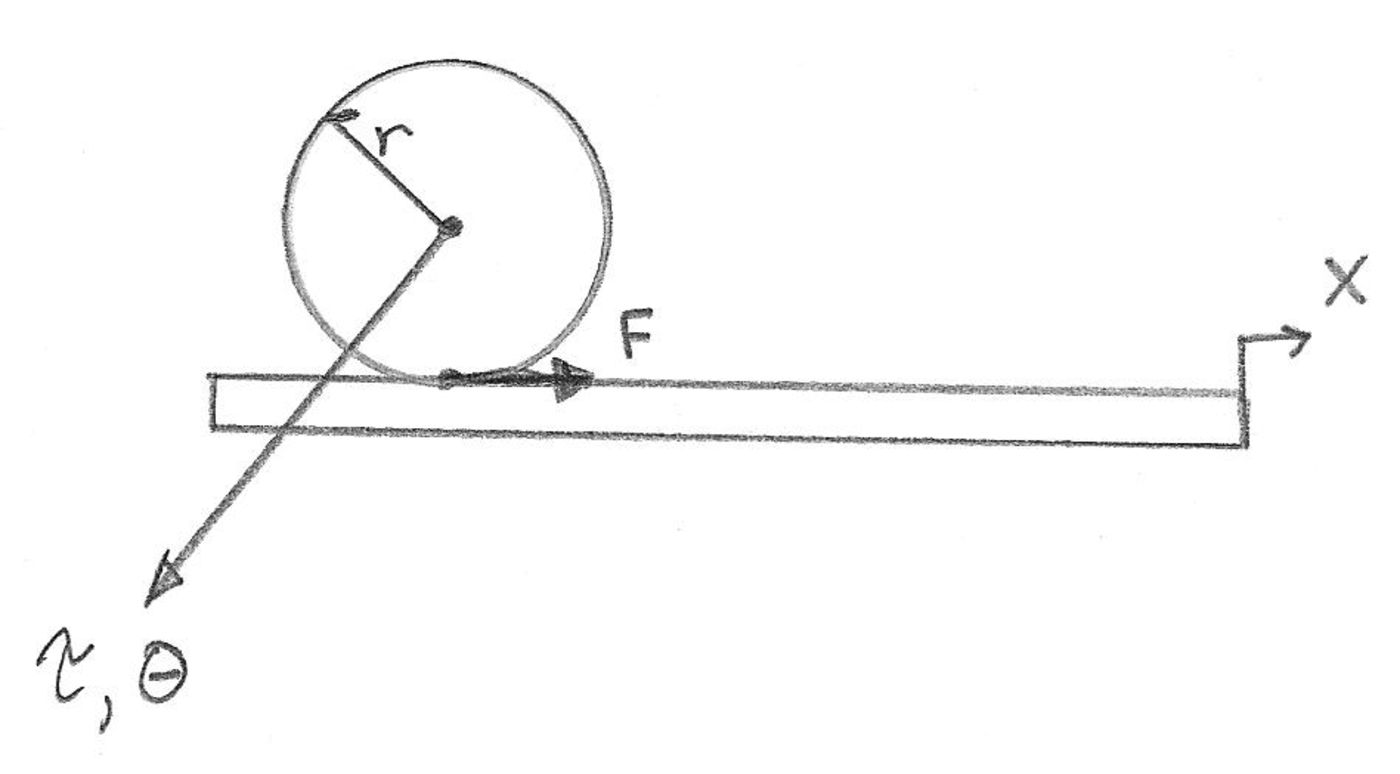
\includegraphics[width=3.5in]{figs03/00755.png}
\caption{Rack and Pinion gear system converts rotary to linear motion and force to torque (and vice versa).}\label{rackpinion}
\end{figure}


%%%%%%%%%%%%%%%%%%%%%%%%%    Examples 

\begin{Example}
For the system below, find  $\frac{\theta_1(s)}{\tau_1(s)}$

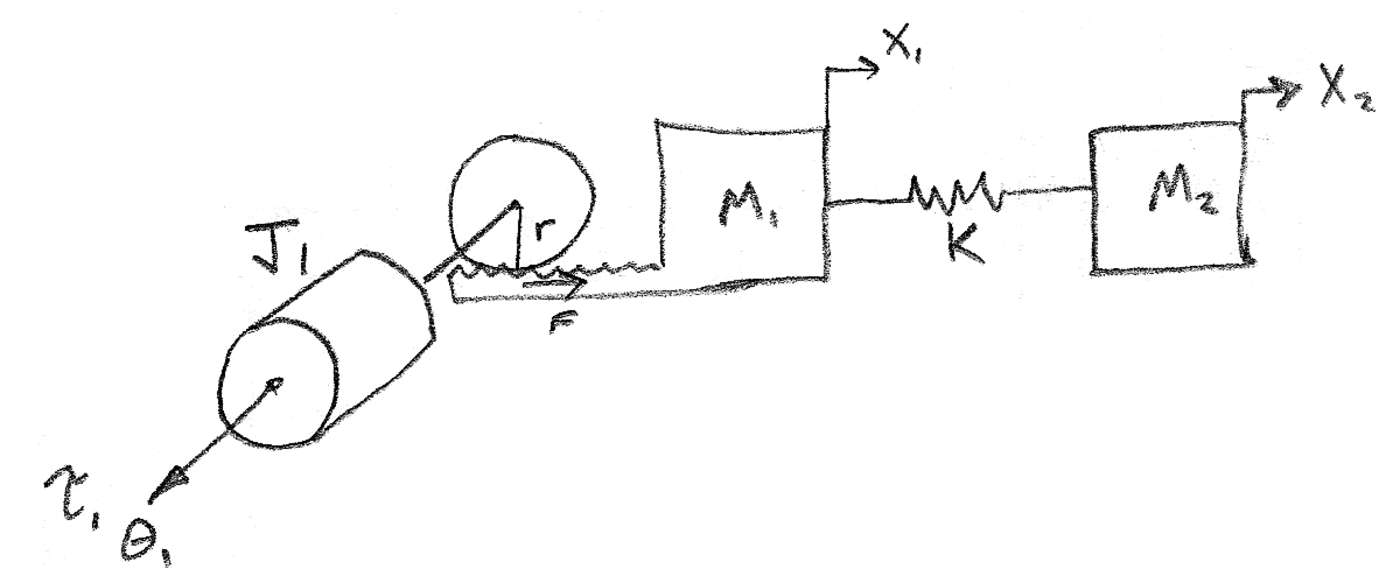
\includegraphics[width=3.5in]{figs03/00754.png}  

The initial EOMS are
\[
J_1\ddot{\theta}_1 + rF = \tau_1     
\]
\[
M_1\ddot{x}_1 + K(x_1-x_2 = F
\]
\[
M_2\ddot{x}_2+K(x_2-x_1)  = 0
\]

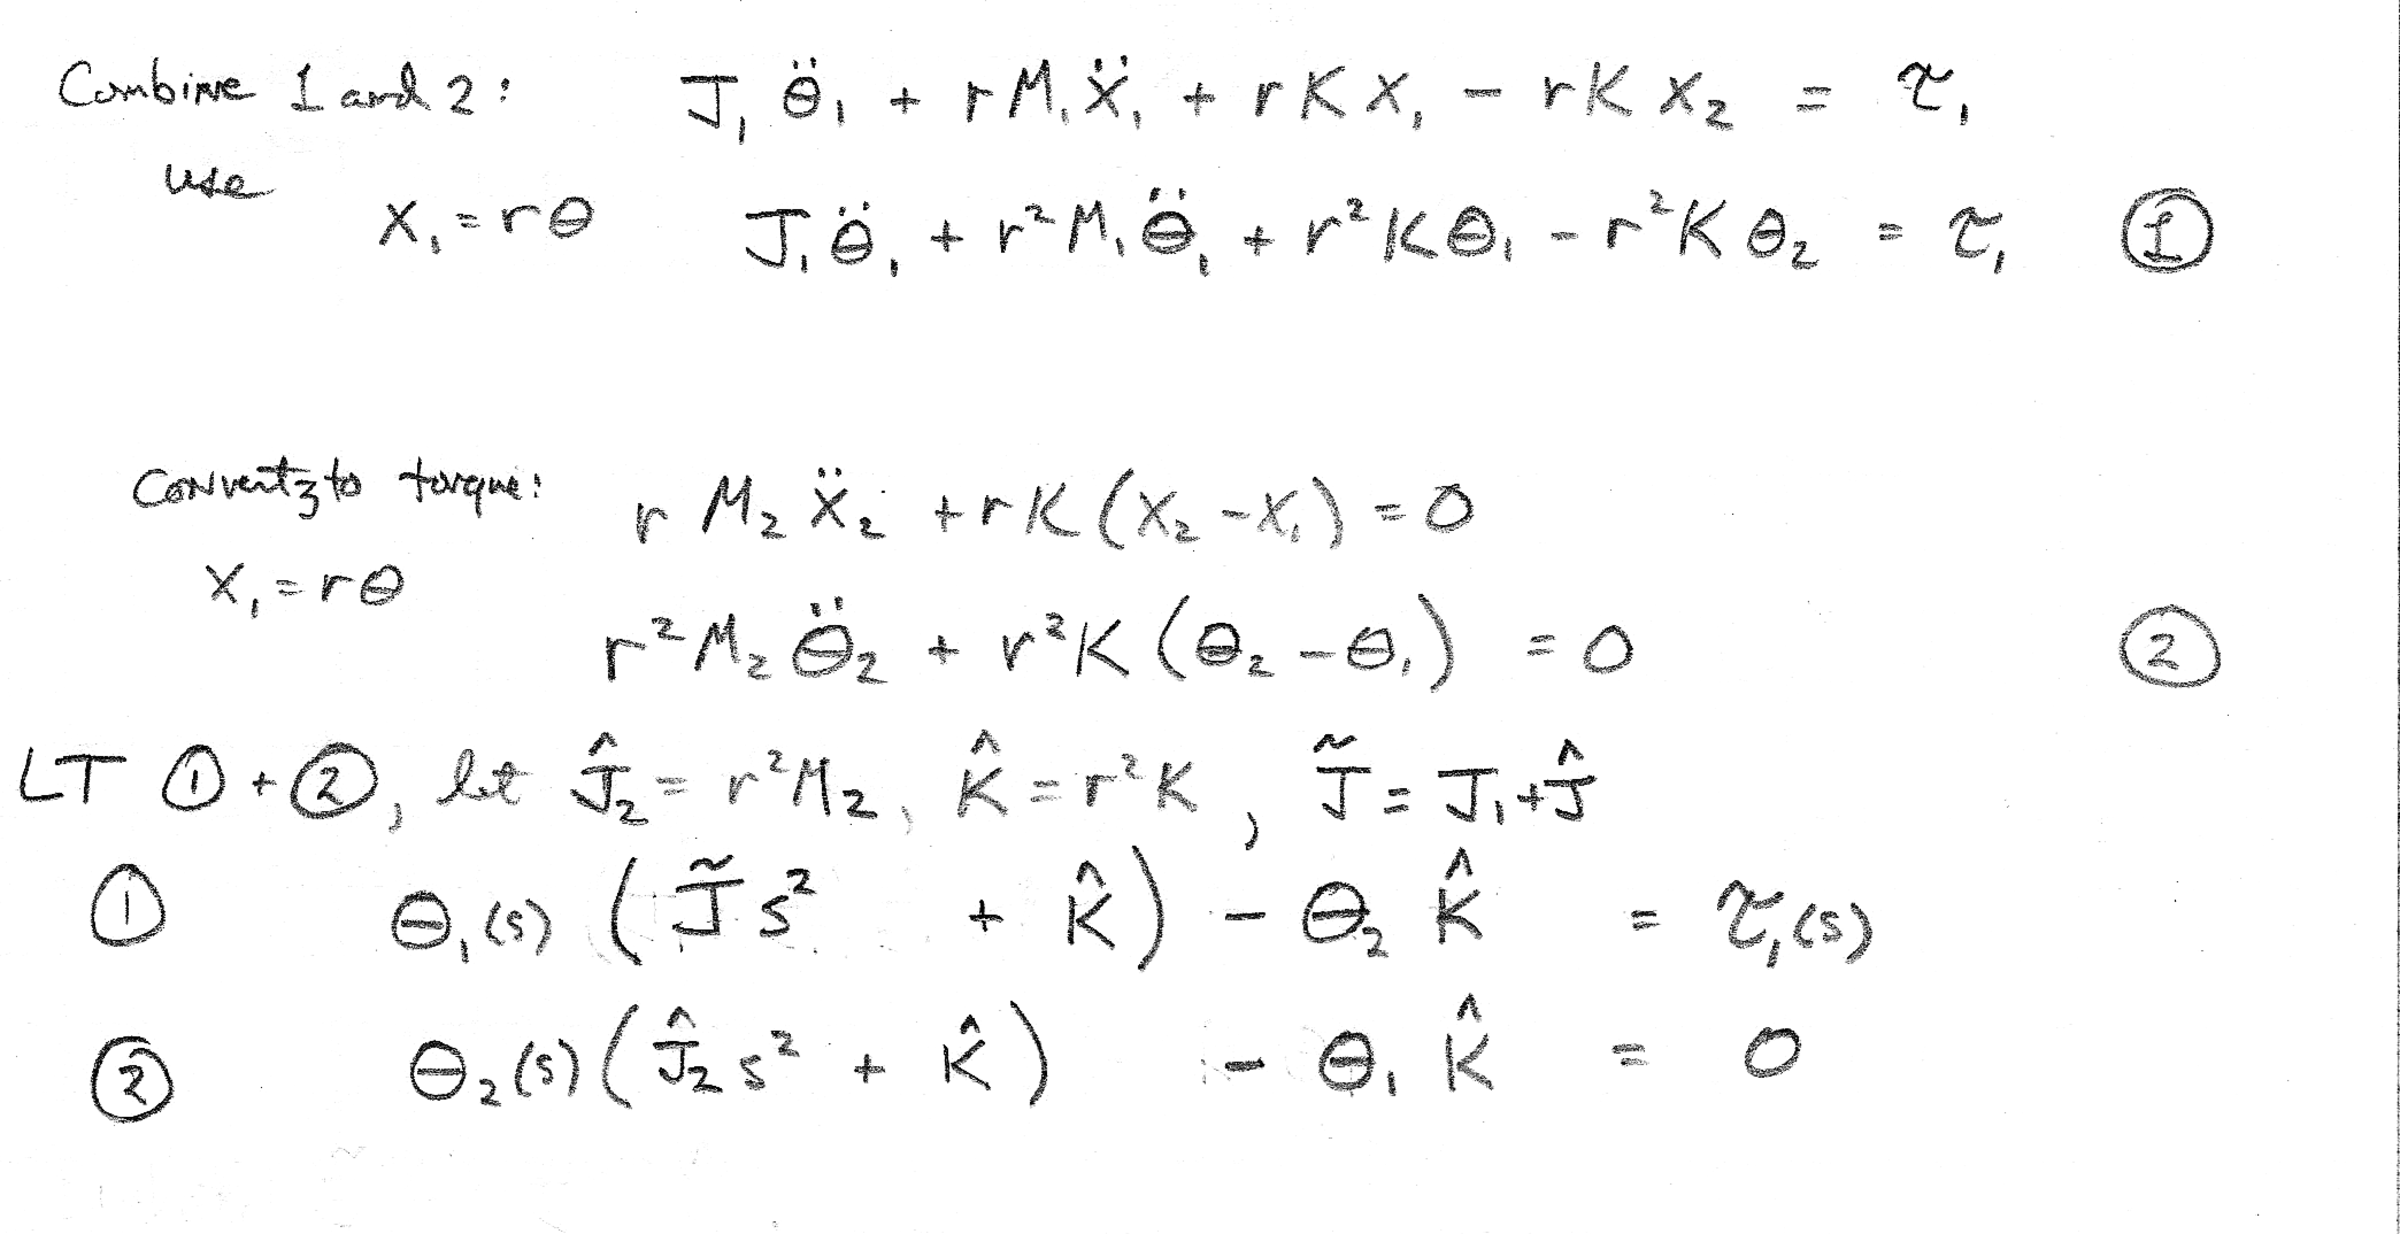
\includegraphics[width=6.0in]{figs03/00756a.png}  

\end{Example}

\begin{ExampleCont}

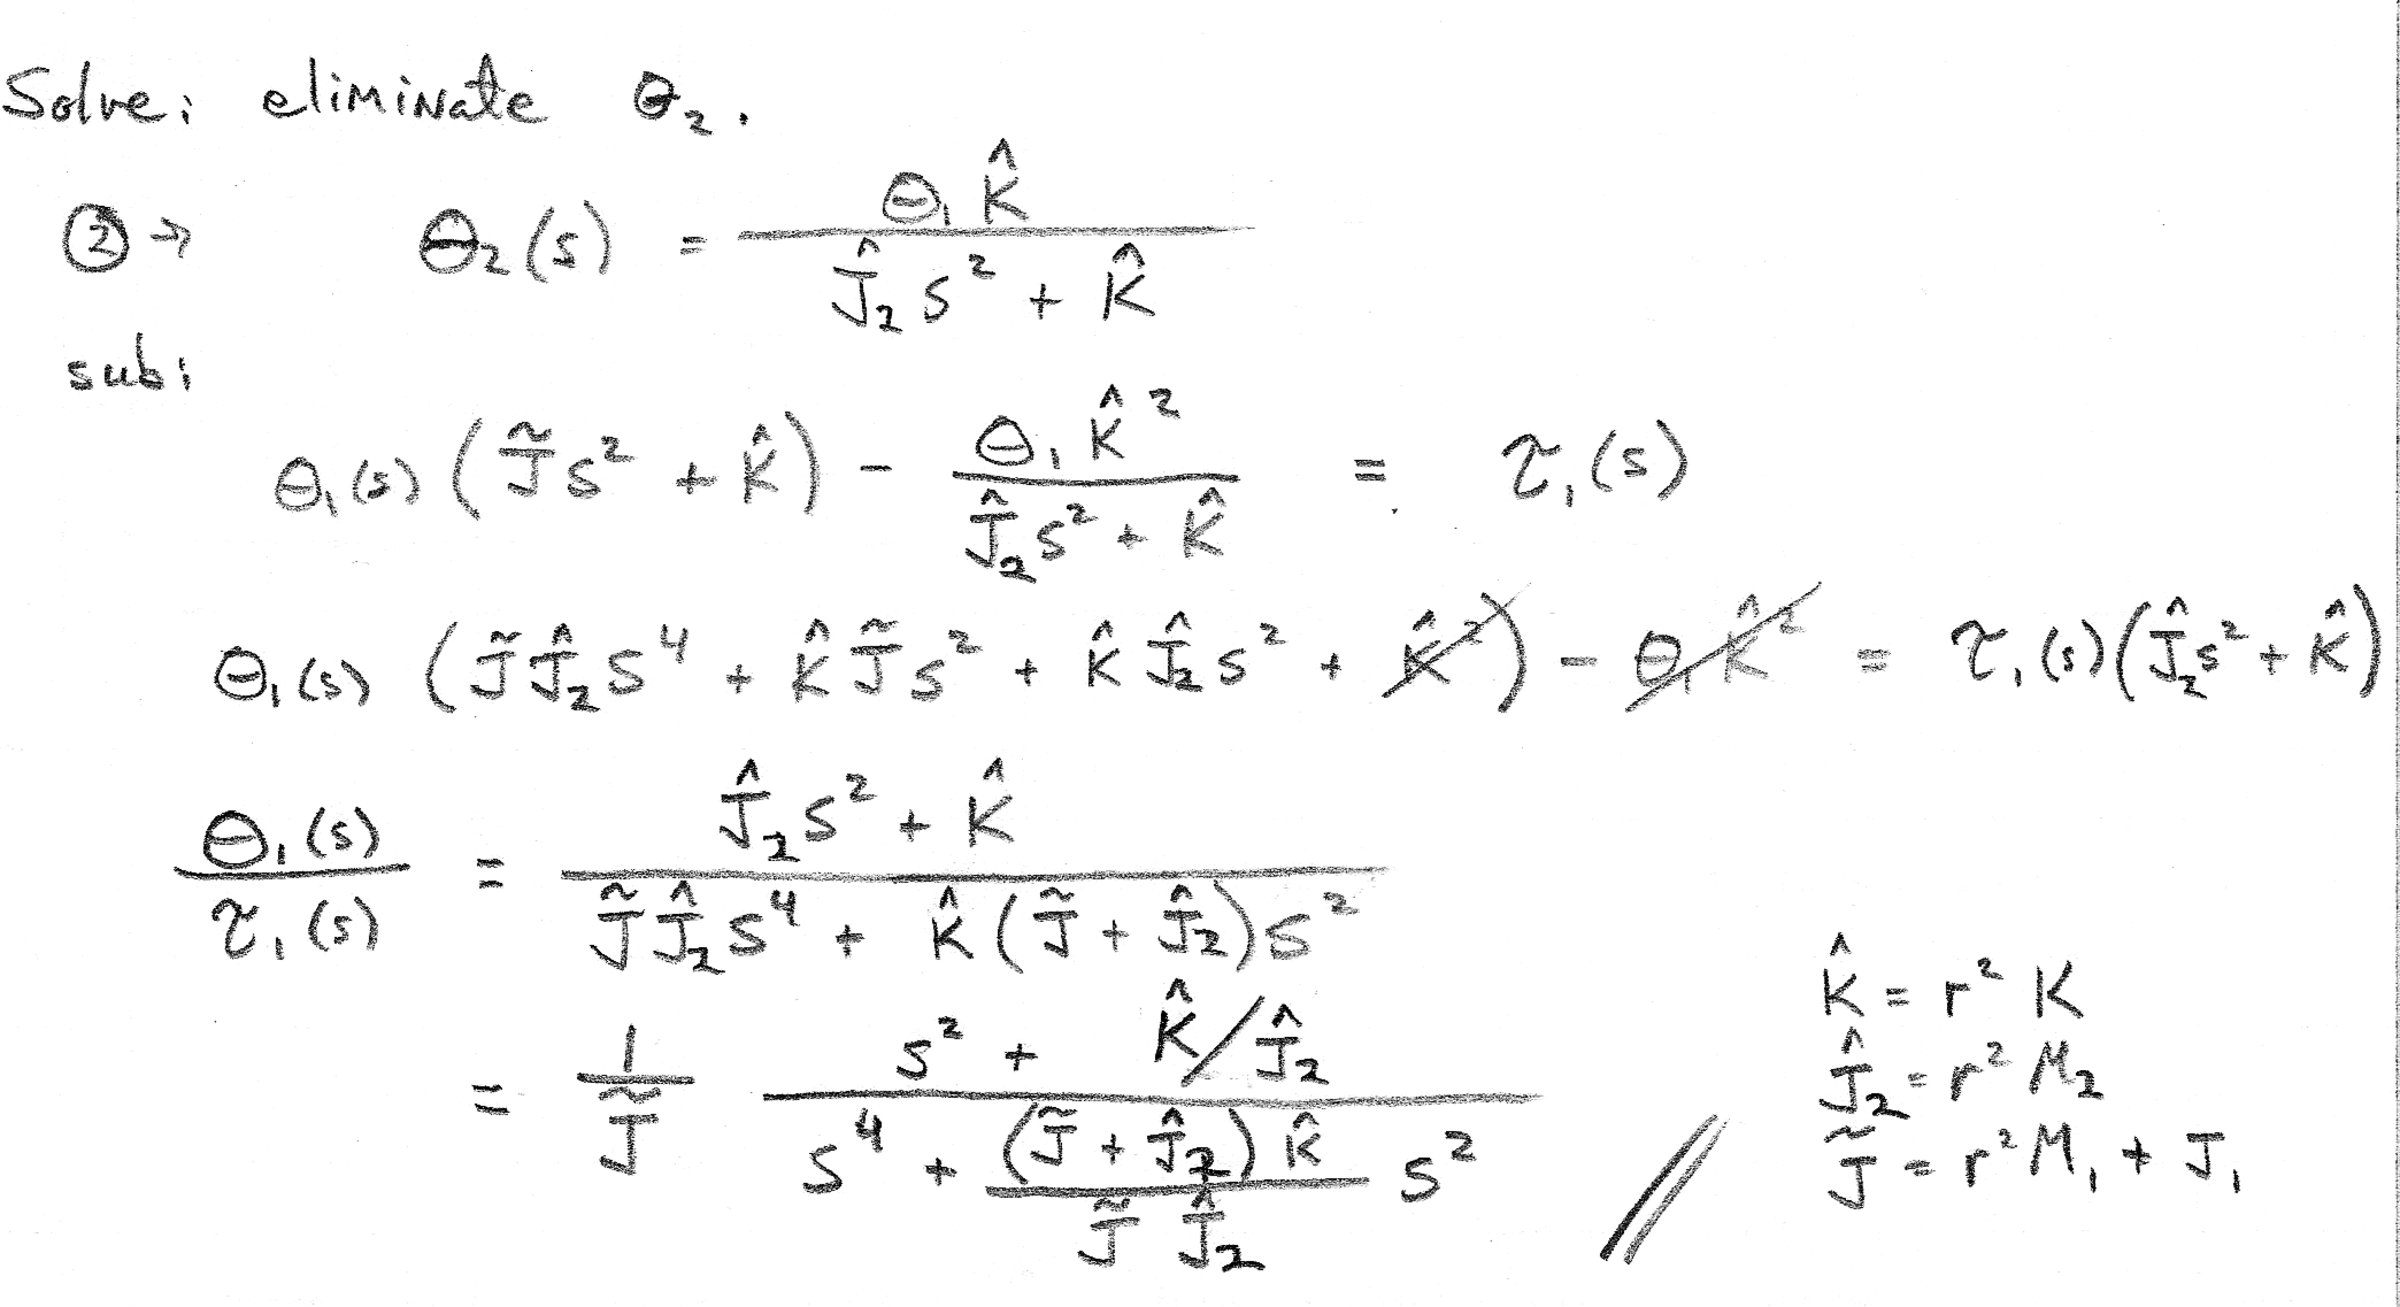
\includegraphics[width=6.0in]{figs03/00756b.png}  

\end{ExampleCont}



